\documentclass[tikz,border=5pt]{standalone}
\usepackage{amsmath}
\usepackage{pgfplots}
\pgfplotsset{compat=1.18}
\usetikzlibrary{arrows.meta,positioning}
\definecolor{ink}{HTML}{16324F}
\definecolor{teal}{HTML}{168A88}
\definecolor{gold}{HTML}{D9892B}
\definecolor{redq}{HTML}{B84A4A}
\begin{document}
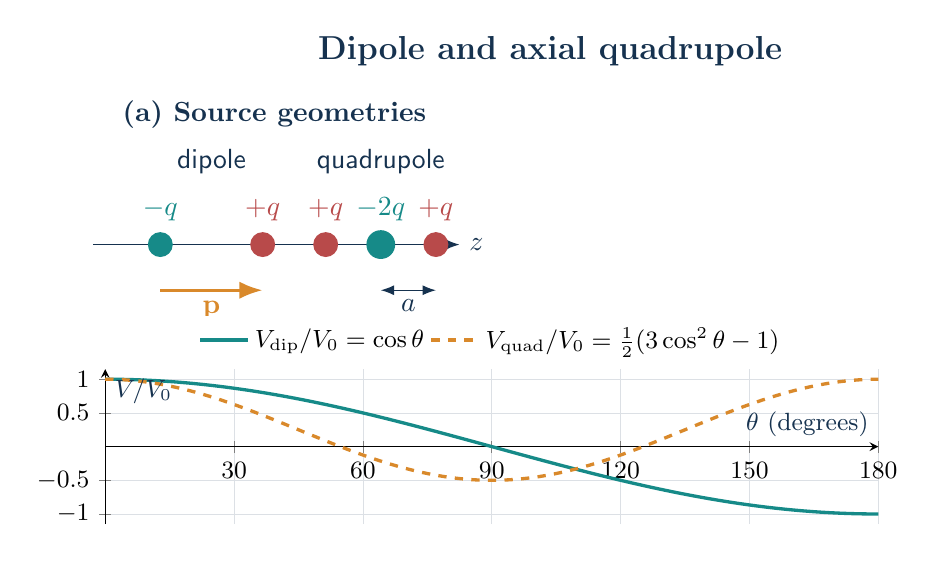
\begin{tikzpicture}[font=\sffamily,>=Latex]
  \node[font=\bfseries\large,ink] at (6.2,6.0) {Dipole and axial quadrupole};

  \begin{scope}[shift={(0.5,3.45)}]
    \node[font=\bfseries,ink] at (2.2,1.75) {(a) Source geometries};
    \draw[ink,->] (-.1,.1)--(4.55,.1) node[right] {$z$};
    \fill[teal] (.75,.1) circle (4.5pt) node[above=5pt,teal] {$-q$};
    \fill[redq] (2.05,.1) circle (4.5pt) node[above=5pt,redq] {$+q$};
    \draw[->,gold,very thick] (.75,-.48)--(2.05,-.48) node[midway,below] {$\mathbf p$};
    \node[ink] at (1.4,1.15) {dipole};

    \fill[redq] (2.85,.1) circle (4.5pt) node[above=5pt,redq] {$+q$};
    \fill[teal] (3.55,.1) circle (5.2pt) node[above=5pt,teal] {$-2q$};
    \fill[redq] (4.25,.1) circle (4.5pt) node[above=5pt,redq] {$+q$};
    \draw[<->,ink] (3.55,-.48)--(4.25,-.48) node[midway,below] {$a$};
    \node[ink] at (3.55,1.15) {quadrupole};
  \end{scope}

  \begin{axis}[
    at={(0.55cm,0cm)},anchor=south west,
    width=11.4cm,height=3.55cm,
    xmin=0,xmax=180,ymin=-1.15,ymax=1.15,
    axis lines=middle,
    xlabel={$\theta$ (degrees)},ylabel={$V/V_0$},
    xtick={0,30,60,90,120,150,180},
    ytick={-1,-.5,0,.5,1},
    grid=both,grid style={line width=.2pt,draw=ink!15},
    tick label style={font=\small},
    label style={font=\small,ink},
    legend style={draw=none,fill=white,font=\small,at={(.5,1.03)},anchor=south,legend columns=2},
    clip=false
  ]
    \addplot[teal,very thick,domain=0:180,samples=241] {cos(x)};
    \addlegendentry{$V_{\rm dip}/V_0=\cos\theta$}
    \addplot[gold,very thick,dashed,domain=0:180,samples=241] {0.5*(3*cos(x)^2-1)};
    \addlegendentry{$V_{\rm quad}/V_0=\tfrac12(3\cos^2\theta-1)$}
  \end{axis}
\end{tikzpicture}
\end{document}
